%!TEX root = ../thesis.tex

%%%%% Chapter: Basic Assumptions %%%%%
\chapter{Basic Assumptions}
\label{chap:basic-assumptions}

\ifpdf
    \graphicspath{{Chapter2/Figs/Raster/}{Chapter2/Figs/PDF/}{Chapter2/Figs/}}
\else
    \graphicspath{{Chapter2/Figs/Vector/}{Chapter2/Figs/}}
\fi

% This chapter states the basic assumptions on the system inputs and output which are used across all other chapters. These assumptions are made in order to simplify the problem. The available lecture data for these project is also identified.

%%% Overview %%%
\section{Overview}

\Cref{fig:sys-diagram-basic} is a simplified diagram which shows the main inputs and output of the desired system. The system takes as inputs a handout file and its corresponding lecture audio file, and outputs the alignment result which maps each chunk of the handout to the corresponding segment (starting time + ending time) of the lecture audio file.

\begin{figure}[!hb]
  \centering
  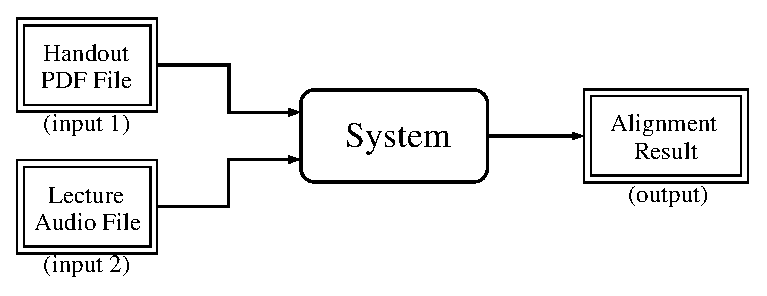
\includegraphics[width=.75\textwidth]{sys-diagram.eps}
  \caption{The inputs and output of the system}
  \label{fig:sys-diagram-basic}
\end{figure}

The handout files are assumed to be in PDF format, but the lecture audio files may take various formats. The alignment output is assumed to be taking the JSON format, which is readable by both human and computers. Additional assumptions on the inputs and output are discussed in the following sections.


%%% Handouts %%%
\section{Handouts}

The handouts are collections of necessary textual and figural information for the purpose of teaching specific courses, which form the crucial part of the system inputs. On Moodle (VLE), almost all uploaded handout files are in PDF format, so it's natural to restrict the input handout file of the system to be taking PDF format.

A proper model of the handouts is required for the purpose of designing the software system. At the first level of abstraction, a handout can be seen as a sequence of images. Each of the images could be further decomposed into basic components like text, equations, tables and figures. These components could be either handwritten or printed.

Since recognising complex components like equations, tables and figures could be really difficult and requires sophisticated algorithms, we will assume that the input handout files contain only text information (printed + handwritten) and will only focus on recognition of text.


%%% Lecture Audio Files %%%
\section{Lecture Audio Files}

The lecture audio file corresponding to the input handout PDF file is another important system input. The format of the input audio files are not particularly specified since we can convert the audio files into any desired format with a proper audio transcoder. Hence we will assume that the input audio files may take any audio format, with the only requirement that this format should be able to be transcoded to any required format in the system.

We shall also make assumptions on how the lecturers deliver lectures. Normally, the lecturers will simply just read and explain handouts sequentially from top to bottom, page by page. However, they may occasionally skip sections or revisit previous sections during the lectures. In order to simplify the task in this project, we assume that the lecturers will refer to the handouts in strictly sequential order when giving lectures.

Another assumption on how the lecturers deliver lectures is that the amount of time spent on explaining a chunk of handout should be roughly proportional to the number of words in that chunk. This is an important assumption which is used in the design of the core alignment algorithm. Again this is actually a huge simplification of the problem and in real lectures this relationship is usually far from linear. 


%%% Alignment Result %%%
\section{Alignment Results}
\label{sec:assume-align-res}

The eventual output of the software system is the alignment result which describes the matches between the chunks of the handout input and the segments of the associated audio file. Technically, any suitable form of text file could be used to describe the alignment result. In this project, the alignment output uses the JSON (JavaScript Object Notation) format since it's well strctured, completely human-readable and easily interpretable by computer programs.

\begin{figure}[!htb]
  \centering
  \begin{subfigure}{.45\textwidth}
    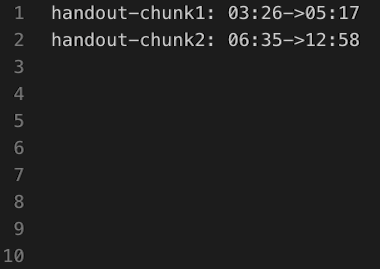
\includegraphics[width=\textwidth]{txt-example.png}
    \caption{Self defined format}
  \end{subfigure}
  \begin{subfigure}{.45\textwidth}
    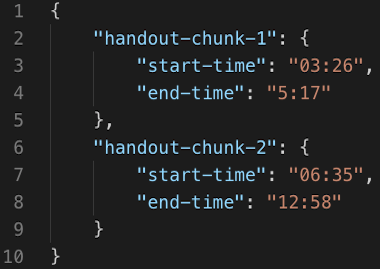
\includegraphics[width=\textwidth]{json-example.png}
    \caption{JSON format of the same information}
  \end{subfigure}
  \caption{Comparison between a self defined format and the JSON format which represent the same information}
  \label{fig:txt-json-compare}
\end{figure}

\Cref{fig:txt-json-compare} compares a piece of text of a self defined format with the JSON representation of the same information. We can notice that the JSON representation is longer but is organised in a more structured way. In addition, there are wide library supports for parsing JSON files in most of the mainstream programming languages (Java, Python, etc).


\section{Available Lecture Data}

Professor Malcolm Smith from the Control Group has kindly provided his full PDF lecture notes of Part IA Mathematics (Easter Term 2010) and all associated video recordings for usage within the scope of the project. The lecture data consists of 2 handout PDF files (41 A4 pages in total) and 7 associated lecture video files (each file roughly hour-long). These available handouts contain a large portion of handwritten notes which agrees with our project aim.

\nomenclature[z-PDF]{PDF}{Portable Document Format}
\nomenclature[z-JSON]{JSON}{JavaScript Object Notation}